%!TEX root =  main.tex
%The sensors are differentiated in terms of their prediction efficiency and cost. 
The goal of this section is to formally introduce the unsupervised linear sensor acquisition problem.
\todoc{Linear = sensors are ordered in a total order.}
Unsupervised sensor acquisition is a partial monitoring problem with a finite action set $\A = [K]$
with $K\ge 2$ being the number of sensors.
A problem instance $\theta = (P,c)$ is specified by an unknown distribution $P$ over 
$\{0,1\}^{K+1}$ and a known cost vector $c\in [0,1]^K$.
In each round, a random binary vector $(\Yt,\Yt^1,\dots,\Yt^K)$ is generated from $P$ in an iid fashion.
The learner's goal in round $t$ is to figure out 
the hidden, stochastic state $Y_t\in \{0,1\}$ of the environment based on the sensor outputs $(\Yt^{k})_{k\in [K]}$.
The dilemma of the learner is which sensors to use for predicting this state.
The learner knows that the sensors are ordered from least to most accurate:
Letting $\gamma_i  =\Prob{\Yt^{i}\ne \Yt}$ be the probability of sensor $i$ being wrong,
$\gamma_1\ge \gamma_2 \ge \dots \ge \gamma_K$.
The learner in each round can decide to observe the outputs of the first $A_t\in \A$ sensors
at the cost of $\sum_{i=1}^{A_t} c_i$.
%The learner never observes the true state $Y_t$ of the environment.
Since the learner knows that the most accurate sensor is the one with the highest index,
the learner uses $Y_t^{A_t}$ to predict $Y_t$.
When the prediction $Y_t^{A_t}$ is incorrect, the learner incurs a unit cost. \todoc{Should we use rewards?!}
Thus, the learner's expected cost in round $t$ upon choosing action $k$ is
$c(k,\theta) = \gamma_k+\sum_{i=1}^k c_i$.
The action that minimizes this cost optimally balances the sensor usage cost with the sensor accuracies.
The learner's expected regret after $n$ rounds is 
\begin{align*}
\Regret_n = \EE{\sum_{t=1}^n c(A_t,\theta)} -\, n \min_{k\in [K]} c(k,\theta)\,.
\end{align*}
Note that the learner never learns about the true state of the environment. 
This lack of feedback easily makes the problem unlearnable, i.e., 
for each learner, there exists some environment $\theta$ such that the learner suffers
maximal regret on $\theta$ and its regret grows linearly with $n$.
The purpose of the next section is to give a characterization of restrictions on the set of environments
that makes learning possible.


\begin{wrapfigure}{r}{5cm}
	\vspace{-.5cm}
	\centering
	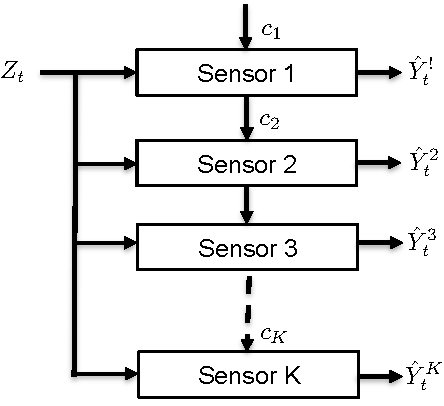
\includegraphics[scale=.6]{../Figures/SensorCascade}
	\caption{Cascade of sensors.
	Each sensor predicts a label $Y_t$ (not shown) associated
	with a random instance $Z_t$. The output of sensor $k$
	can be acquired at the additional cost $c_{k-1}>0$ after 
	the output of sensor has been acquired. Sensors with higher indices
	have a smaller probability of missing the true label.
	\todoc[inline]{I kept the figure, but the figure should be updated to better reflect
	the current problem description.}
	}\label{wrap-fig:1}
	\vspace{-.5cm}
\end{wrapfigure} 

